\documentclass[10pt,twocolumn]{article}
\usepackage[letterpaper,margin=0.7in,columnsep=0.25in]{geometry}
\usepackage[T1]{fontenc}
\usepackage{lmodern,microtype}
\usepackage{amsmath,booktabs,graphicx,xcolor}
\usepackage[hidelinks]{hyperref}
\usepackage[numbers,sort&compress]{natbib}
\usepackage{caption}
\captionsetup{font=small,labelfont=bf,skip=4pt}
\setlength{\textfloatsep}{8pt plus 2pt minus 2pt}
\setlength{\dbltextfloatsep}{8pt plus 2pt minus 2pt}
\graphicspath{{../results/analysis/figures/}}

% All numbers below come from generated/numbers.tex and generated/tab_*.tex, written by
% `raterbench report-assets` from the saved run outputs. Do not type results by hand.
% Generated by `raterbench report-assets`; do not edit.
\newcommand{\accBestDr}{81.8}
\newcommand{\accBestTe}{73.9}
\newcommand{\accFtDr}{82.1}
\newcommand{\accFtTe}{69.4}
\newcommand{\aurocLpMax}{0.80}
\newcommand{\aurocLpMin}{0.69}
\newcommand{\aurocScMax}{0.58}
\newcommand{\aurocScMin}{0.54}
\newcommand{\aurocVerbMax}{0.77}
\newcommand{\aurocVerbMin}{0.52}
\newcommand{\bestCondDr}{codebook}
\newcommand{\bestCondTe}{codebook}
\newcommand{\bestModelDr}{Qwen 2.5 7B}
\newcommand{\bestModelTe}{Llama 3.1 8B}
\newcommand{\cpAllErrDr}{18.2}
\newcommand{\cpAllErrTe}{26.1}
\newcommand{\cpAutoErrDr}{13.0}
\newcommand{\cpAutoErrTe}{14.0}
\newcommand{\cpCovDr}{0.890}
\newcommand{\cpCovTe}{0.939}
\newcommand{\cpFtAutoErrDr}{13.5}
\newcommand{\cpFtAutoErrTe}{12.6}
\newcommand{\cpFtRoutedDr}{16}
\newcommand{\cpFtRoutedTe}{60}
\newcommand{\cpModelDr}{Qwen 2.5 7B}
\newcommand{\cpModelTe}{Llama 3.1 8B}
\newcommand{\cpRoutedDr}{15}
\newcommand{\cpRoutedTe}{56}
\newcommand{\errAmbiguousGoldDr}{13}
\newcommand{\errAmbiguousGoldTe}{14}
\newcommand{\errAmbiguousGoldTotal}{27}
\newcommand{\errImplicitStanceDr}{8}
\newcommand{\errImplicitStanceTe}{7}
\newcommand{\errKeywordRelianceDr}{0}
\newcommand{\errKeywordRelianceTe}{3}
\newcommand{\errLabelBoundaryDr}{20}
\newcommand{\errLabelBoundaryTe}{4}
\newcommand{\errMissingContextDr}{0}
\newcommand{\errMissingContextTe}{2}
\newcommand{\errNCoded}{100}
\newcommand{\errNDr}{50}
\newcommand{\errNTe}{50}
\newcommand{\errNegationDr}{2}
\newcommand{\errNegationTe}{0}
\newcommand{\errOtherDr}{2}
\newcommand{\errOtherTe}{0}
\newcommand{\errOverInferenceDr}{5}
\newcommand{\errOverInferenceTe}{8}
\newcommand{\errSarcasmIronyDr}{0}
\newcommand{\errSarcasmIronyTe}{7}
\newcommand{\errStatus}{drafted with a language model and reviewed by the author}
\newcommand{\errTargetConfusionDr}{0}
\newcommand{\errTargetConfusionTe}{5}
\newcommand{\errTopNDr}{20}
\newcommand{\errTopNTe}{14}
\newcommand{\errTopNameDr}{label boundary}
\newcommand{\errTopNameTe}{ambiguous gold}
\newcommand{\flipGenderMax}{3.3}
\newcommand{\flipGenderMin}{1.7}
\newcommand{\flipParaMax}{9.0}
\newcommand{\flipParaMin}{6.9}
\newcommand{\flipTypoMax}{8.0}
\newcommand{\flipTypoMin}{2.9}
\newcommand{\kappaBestCIDr}{[0.58, 0.69]}
\newcommand{\kappaBestCITe}{[0.52, 0.61]}
\newcommand{\kappaBestDr}{0.64}
\newcommand{\kappaBestTe}{0.56}
\newcommand{\kappaFtDr}{0.64}
\newcommand{\kappaFtSeedsDr}{0.62 $\pm$ 0.02}
\newcommand{\kappaFtSeedsTe}{0.48 $\pm$ 0.01}
\newcommand{\kappaFtTe}{0.49}
\newcommand{\kappaZsRangeDr}{0.48--0.53}
\newcommand{\kappaZsRangeTe}{0.34}
\newcommand{\nCalDr}{305}
\newcommand{\nCalTe}{249}
\newcommand{\nCalls}{40,842}
\newcommand{\nConfCells}{56}
\newcommand{\nConfOk}{56}
\newcommand{\nEvalDr}{715}
\newcommand{\nEvalTe}{1,000}
\newcommand{\nParseFail}{1}
\newcommand{\nSigTests}{48}
\newcommand{\pBestVsFtDr}{=1.00}
\newcommand{\pBestVsFtTe}{=0.14}
\newcommand{\pLlamaQwenCbDr}{<0.001}
\newcommand{\pLlamaQwenCbTe}{<0.001}
\newcommand{\pZsCbTeMax}{<0.001}
\newcommand{\pZsVsFtMax}{=0.046}
\newcommand{\runHours}{3.6}
\newcommand{\scRoutedMin}{100}
\newcommand{\sgGapFtDr}{0.12}
\newcommand{\sgGapFtTe}{0.09}
\newcommand{\sgGapLlamaDr}{0.18}
\newcommand{\sgGapLlamaTe}{0.14}
\newcommand{\sgGapQwenDr}{0.16}
\newcommand{\sgGapQwenTe}{0.23}
\newcommand{\sgPFtDr}{=0.069}
\newcommand{\sgPFtTe}{<0.001}
\newcommand{\sgPLlamaDr}{<0.001}
\newcommand{\sgPLlamaTe}{=0.11}
\newcommand{\sgPQwenDr}{=0.020}
\newcommand{\sgPQwenTe}{=0.050}
\newcommand{\verbDistinctMax}{6}
\newcommand{\verbRoutedTeMin}{88}


% error coding done


\newcommand{\authorname}{SisnuSK}

\title{\textbf{RaterBench: How Reliable Are Small Open LLMs\\as Expert Text Annotators?}}
\author{\authorname}
\date{}

\begin{document}
\maketitle

\begin{abstract}
More and more researchers ask large language models (LLMs) to label text that trained annotators
used to label. I test how far that can be trusted on two public social-media tasks: stress in
Reddit posts (Dreaddit) and stance in tweets (TweetEval). Two open 7--8B models, Llama~3.1 and
Qwen~2.5, labeled every item under four prompting strategies, and I compared them with a
fine-tuned RoBERTa model using the statistics normally used for inter-rater reliability, with
bootstrap confidence intervals. With its best prompt, each LLM agrees with the gold labels about
as well as the fine-tuned model does (Cohen's $\kappa$ \kappaBestDr{} vs.\ \kappaFtDr{} on
Dreaddit, \kappaBestTe{} vs.\ \kappaFtTe{} on TweetEval). Zero-shot prompting falls well short,
and the better model depends on the task. Of three confidence signals, only token probabilities
separate right from wrong answers usefully. Split conformal triage built on them sends
\cpRoutedDr\% of Dreaddit items to a human at a 90\% coverage target, but \cpRoutedTe\% of
stance items. Labels also change under \flipParaMin--\flipParaMax\% of meaning-preserving
paraphrases. The code, prompts and fixed sample IDs are public.
\end{abstract}

\section{Introduction}
Labeling text by hand is slow and expensive, so it is no surprise that researchers in
psychiatry, public health and computational social science have started handing the job to
LLMs. The worry is that the models make mistakes quietly and systematically. Before relying on
LLM labels, a researcher would want to know four things. How closely do they agree with expert
labels (RQ1)? Does the model's confidence say which labels to trust (RQ2)? Can that confidence
decide which items still need a human, with a guaranteed coverage level (RQ3)? And do the errors
cluster in particular subgroups, or change when the wording changes but the meaning does not
(RQ4)?

RaterBench answers these with the tools used to judge human annotators: Cohen's
$\kappa$~\cite{cohen1960kappa} and Krippendorff's $\alpha$~\cite{krippendorff2004content} with
95\% bootstrap intervals, paired McNemar tests~\cite{mcnemar1947} with Holm
correction~\cite{holm1979}, standard calibration metrics~\cite{guo2017calibration}, and split
conformal prediction~\cite{angelopoulos2021gentle}. Every number in this report is produced by
scripts in the repository from cached model outputs.

\section{Related work}
\emph{[To be written: LLMs as annotators in the social sciences; uncertainty and calibration of
LLMs; conformal prediction for classification; robustness and bias audits of text
classifiers.]}

\section{Data and setup}
\paragraph{Datasets.} \emph{Dreaddit}~\cite{turcan2019dreaddit} contains excerpts of Reddit
posts from ten subreddits (grouped into five domains), labeled stress or not stress by crowd
workers, whose own agreement was moderate (Fleiss' $\kappa=0.47$ in the original paper).
\emph{TweetEval stance}~\cite{barbieri2020tweeteval}, which comes from SemEval-2016
Task~6~\cite{mohammad2016semeval}, labels tweets as favoring, opposing, or taking no stance on one
of five targets. I evaluate on fixed stratified samples of the test splits (\nEvalDr{} Dreaddit
and \nEvalTe{} TweetEval items). Conformal prediction gets its own calibration set that never
overlaps the evaluation set: the remaining \nCalTe{} TweetEval test items, and \nCalDr{} items
held out from Dreaddit's training split, because its test split was too small to divide.
Few-shot examples are drawn only from training data.

\paragraph{Models and prompts.} Llama~3.1~8B Instruct and Qwen~2.5~7B Instruct, both 4-bit and
served by Ollama, labeled every item under four prompts. \emph{Zero-shot} gives the task and the
label definitions. \emph{Few-shot} adds five label-balanced training examples. \emph{Codebook}
replaces them with a detailed annotation guideline covering inclusion rules and edge cases, and
\emph{codebook+reason} also asks for a short rationale before the label. The models answer in
JSON with a label and a 0--100 confidence, and a malformed answer gets one corrective retry. Main
runs use temperature~0. Producing all \nCalls{} labels took \runHours{} hours on one laptop GPU,
and only \nParseFail{} answer could not be parsed (it counts as an error). The baselines are the
majority class and RoBERTa-base~\cite{liu2019roberta} fine-tuned on the training split. I trained
it with three seeds and report seed~13 with bootstrap intervals; across seeds its $\kappa$ is
\kappaFtSeedsDr{} on Dreaddit and \kappaFtSeedsTe{} on TweetEval.

\paragraph{Confidence signals.} With the codebook prompt I compare three signals:
\emph{verbalized} confidence, the number the model reports; \emph{token probability}, the product
of the probabilities of the tokens that spell the label; and
\emph{self-consistency}~\cite{wang2023selfconsistency}, the share of five extra answers sampled
at temperature~0.7 that agree with the temperature-0 label.

\paragraph{Conformal triage.} On the calibration set I fit split-conformal prediction sets with
the LAC score~\cite{sadinle2019lac}; adaptive prediction sets~\cite{romano2020aps} are in the
repository too. An item whose set contains exactly one label is labeled automatically, and
everything else goes to a human. The LLMs only give a probability for the label they chose, so
the rest of the probability is spread evenly over the other labels.

\section{Results}

\begin{table*}[t]
\centering\small
\begin{tabular}{llcccc}
\toprule
 & & \multicolumn{2}{c}{Dreaddit (stress)} & \multicolumn{2}{c}{TweetEval (stance)} \\
\cmidrule(lr){3-4}\cmidrule(lr){5-6}
Model & Prompt & $\kappa$ [95\% CI] & F1 & $\kappa$ [95\% CI] & F1 \\
\midrule
Majority class & -- & 0.00 [0.00, 0.00] & 0.34 & 0.00 [0.00, 0.00] & 0.24 \\
RoBERTa-base (fine-tuned) & -- & 0.64 [0.58, 0.69] & 0.82 & 0.49 [0.44, 0.53] & 0.66 \\
\midrule
Llama 3.1 8B & zero-shot & 0.48 [0.42, 0.54] & 0.73 & 0.34 [0.31, 0.38] & 0.54 \\
 & few-shot & 0.46 [0.40, 0.52] & 0.72 & 0.49 [0.44, 0.53] & 0.66 \\
 & codebook & 0.46 [0.41, 0.52] & 0.72 & \textbf{0.56} [0.52, 0.61] & 0.71 \\
 & codebook+reason & 0.50 [0.44, 0.56] & 0.74 & 0.51 [0.46, 0.55] & 0.65 \\
\midrule
Qwen 2.5 7B & zero-shot & 0.53 [0.47, 0.59] & 0.76 & 0.34 [0.30, 0.38] & 0.53 \\
 & few-shot & 0.56 [0.50, 0.61] & 0.77 & 0.44 [0.40, 0.48] & 0.63 \\
 & codebook & \textbf{0.64} [0.58, 0.69] & 0.82 & 0.46 [0.41, 0.50] & 0.64 \\
 & codebook+reason & 0.61 [0.55, 0.67] & 0.81 & 0.49 [0.45, 0.54] & 0.66 \\
\bottomrule
\end{tabular}

\caption{Agreement with gold labels on the evaluation sets (Cohen's $\kappa$ with 95\% bootstrap
CIs over items; macro-F1). Bold: best LLM configuration per dataset. Krippendorff's $\alpha$
tracks $\kappa$ closely and is reported in the repository.}
\label{tab:main}
\end{table*}

\paragraph{RQ1: Agreement.} The prompt turns out to matter about as much as the model
(Table~\ref{tab:main}, Figure~\ref{fig:prompting}). With the right prompt, each LLM catches up
with the fine-tuned baseline on one task: \bestModelDr{} with the codebook on Dreaddit (accuracy
\accBestDr\% against \accFtDr\%, Holm-adjusted McNemar $p\pBestVsFtDr$), and \bestModelTe{} with
the codebook on TweetEval (\accBestTe\% against \accFtTe\%, $p\pBestVsFtTe$). Zero-shot prompting
is significantly worse than the fine-tuned model for both models on both tasks (largest adjusted
$p\pZsVsFtMax$). Stance shows the gap most clearly: zero-shot $\kappa$ is only
\kappaZsRangeTe{}, and the codebook improves both models ($p\pZsCbTeMax$). The two models are
good at different things. With the codebook, Qwen is better on stress ($p\pLlamaQwenCbDr$) and
Llama on stance ($p\pLlamaQwenCbTe$). Asking for reasoning first helped in two of the four
model--task pairs and hurt in the other two.

\begin{figure}[t]
\centering
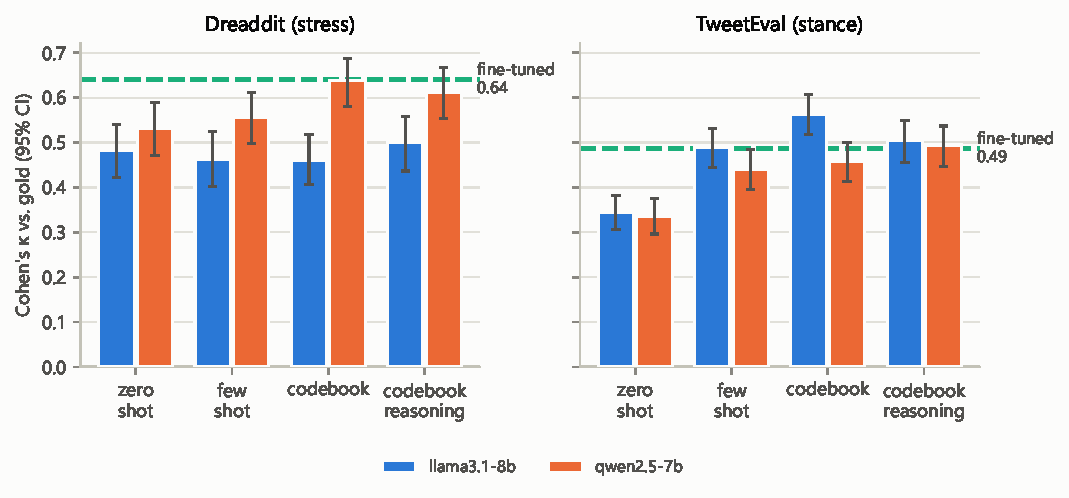
\includegraphics[width=\columnwidth]{fig2_prompting_effect.pdf}
\caption{Cohen's $\kappa$ by prompting strategy (95\% CIs). Dashed line: fine-tuned RoBERTa.}
\label{fig:prompting}
\end{figure}

\paragraph{RQ2: Calibration.} Table~\ref{tab:calib} compares the three signals. Token probability
ranks right and wrong answers most consistently (AUROC \aurocLpMin--\aurocLpMax), even though its
values are poorly calibrated in absolute terms. Verbalized confidence is coarse: no model used
more than \verbDistinctMax{} distinct values on a task, and its AUROC ranges from \aurocVerbMin,
barely above chance, to \aurocVerbMax. A low ECE can hide this. Qwen's verbalized confidence on
Dreaddit is well calibrated on average but hardly distinguishes its errors. Self-consistency
helps even less (AUROC \aurocScMin--\aurocScMax): at temperature~0.7 the extra samples almost
always repeat the first answer, so the models seem to make their mistakes consistently rather
than at random.

\begin{table}[t]
\centering\small\setlength{\tabcolsep}{4pt}
\resizebox{\columnwidth}{!}{\begin{tabular}{llcccc}
\toprule
 & & \multicolumn{2}{c}{Dreaddit} & \multicolumn{2}{c}{TweetEval} \\
\cmidrule(lr){3-4}\cmidrule(lr){5-6}
Model & Signal & ECE$\downarrow$ & AUROC$\uparrow$ & ECE$\downarrow$ & AUROC$\uparrow$ \\
\midrule
Llama 3.1 8B & verbalized & 0.17 & 0.77 & 0.11 & 0.52 \\
 & token prob. & 0.22 & 0.75 & 0.17 & 0.69 \\
 & self-consistency & 0.24 & 0.56 & 0.22 & 0.58 \\
Qwen 2.5 7B & verbalized & 0.05 & 0.55 & 0.18 & 0.53 \\
 & token prob. & 0.16 & 0.80 & 0.29 & 0.71 \\
 & self-consistency & 0.17 & 0.56 & 0.30 & 0.54 \\
RoBERTa-base & softmax & 0.14 & 0.76 & 0.17 & 0.72 \\
\bottomrule
\end{tabular}
}
\caption{Calibration of confidence signals (codebook prompt, eval sets).}
\label{tab:calib}
\end{table}

\paragraph{RQ3: Conformal triage.} At a 90\% coverage target (Table~\ref{tab:conformal}),
\cpModelDr's token probabilities send \cpRoutedDr\% of Dreaddit items to a human. The items it
labels automatically have \cpAutoErrDr\% errors, against \cpAllErrDr\% if it labeled everything,
which is close to what the fine-tuned model achieves (\cpFtRoutedDr\% routed, \cpFtAutoErrDr\%
errors). Stance is much harder: even the best LLM sends \cpRoutedTe\% of items to a human. Coarse
signals make triage pointless. Self-consistency sends \scRoutedMin\% of items to a human in every
setting, and verbalized confidence at least \verbRoutedTeMin\% on stance. Empirical coverage
stayed within the expected finite-sample range in all \nConfOk{} of \nConfCells{}
settings~\cite{vovk2012conditional}. It is worth being clear about what is guaranteed, though:
the coverage of the \emph{set}, not the error rate among auto-labeled items, which can be higher
than the miscoverage level.

\begin{table}[t]
\centering\small\setlength{\tabcolsep}{3pt}
\resizebox{\columnwidth}{!}{\begin{tabular}{llcccccc}
\toprule
 & & \multicolumn{3}{c}{Dreaddit} & \multicolumn{3}{c}{TweetEval} \\
\cmidrule(lr){3-5}\cmidrule(lr){6-8}
Model & Signal & Cov. & Human\% & Err.\% & Cov. & Human\% & Err.\% \\
\midrule
Llama 3.1 8B & token prob. & 0.890 & 33 & 16.4 & 0.939 & 56 & 14.0 \\
 & verbalized & 0.968 & 60 & 8.1 & 0.963 & 88 & 30.6 \\
 & self-consistency & 1.000 & 100 & -- & 1.000 & 100 & -- \\
Qwen 2.5 7B & token prob. & 0.890 & 15 & 13.0 & 0.943 & 61 & 14.7 \\
 & verbalized & 1.000 & 92 & 0.0 & 0.988 & 93 & 16.9 \\
 & self-consistency & 1.000 & 100 & -- & 1.000 & 100 & -- \\
RoBERTa-base & softmax & 0.887 & 16 & 13.5 & 0.927 & 60 & 12.6 \\
\bottomrule
\end{tabular}
}
\caption{LAC conformal triage at 90\% target coverage (codebook prompt). Cov.: empirical
coverage; Human\%: items routed to a human; Err.\%: error on auto-labeled items.}
\label{tab:conformal}
\end{table}

\begin{figure*}[t]
\centering
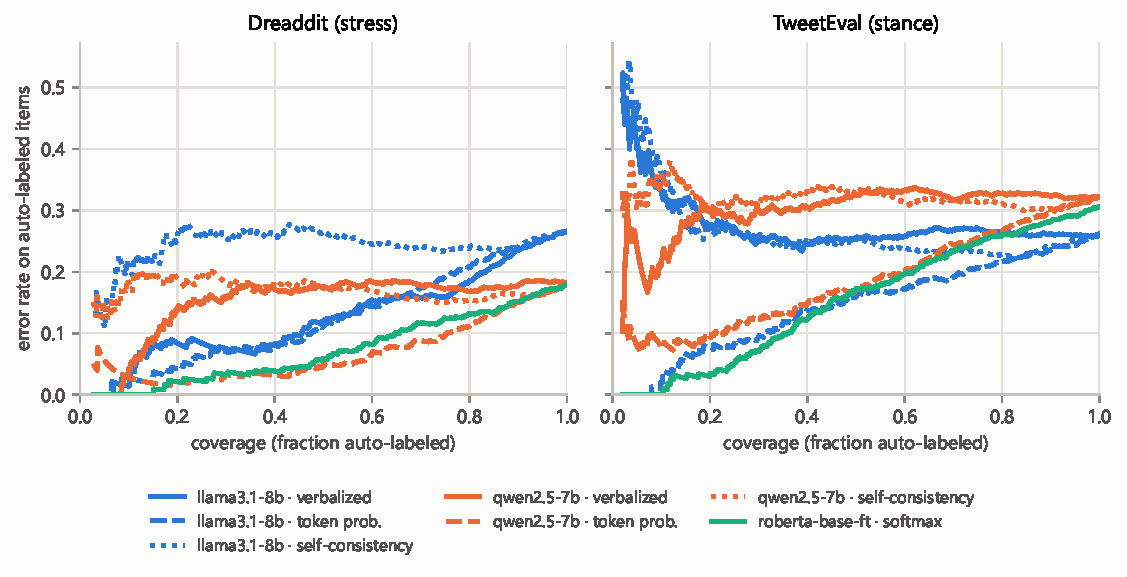
\includegraphics[width=0.49\textwidth]{fig5_risk_coverage.pdf}\hfill
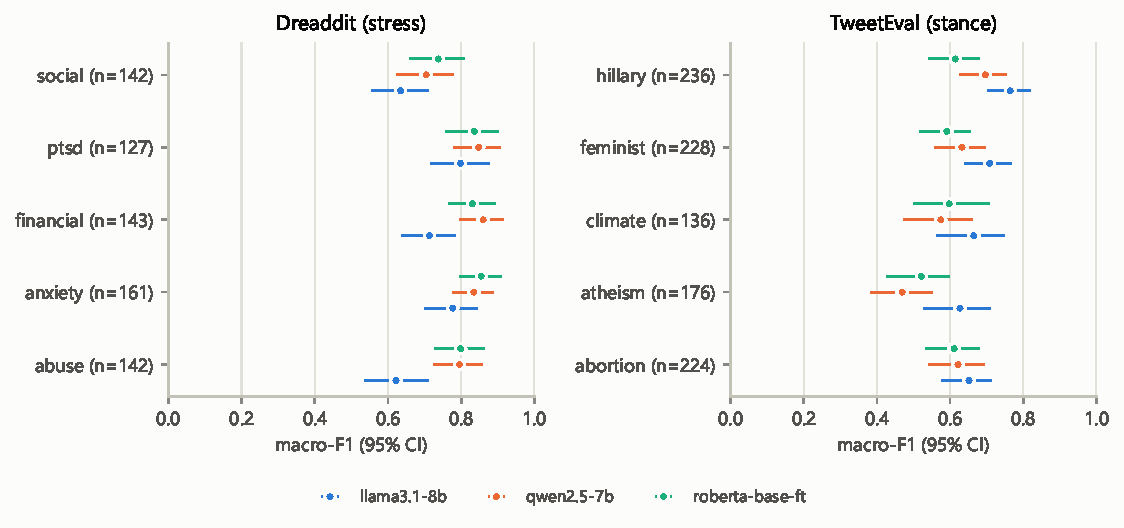
\includegraphics[width=0.49\textwidth]{fig7_subgroups.pdf}
\caption{Left: risk--coverage curves (error among auto-labeled items as more items are
auto-labeled, most confident first). Right: macro-F1 per Dreaddit domain and TweetEval target
(codebook prompt, 95\% CIs).}
\label{fig:rc}
\end{figure*}

\paragraph{RQ4: Subgroups and robustness.} On Dreaddit, both LLMs make errors at different rates
across domains ($\chi^2$ test, $p\sgPLlamaDr$ for Llama and $p\sgPQwenDr$ for Qwen, with macro-F1
gaps of up to \sgGapLlamaDr{} and \sgGapQwenDr), while the fine-tuned model does not
significantly ($p\sgPFtDr$). TweetEval shows the opposite pattern. There the fine-tuned model's
errors vary across targets ($p\sgPFtTe$) and the LLMs' less clearly ($p\sgPLlamaTe$,
$p\sgPQwenTe$; Figure~\ref{fig:rc}). These groups are topics and communities, not demographic
groups, and they differ in size and label mix. Edits that keep the meaning still change labels
(Table~\ref{tab:perturb}). Across both models and the zero-shot and codebook prompts, labels flip
for \flipGenderMin--\flipGenderMax\% of gender-swapped Dreaddit posts,
\flipTypoMin--\flipTypoMax\% of items with typos, and \flipParaMin--\flipParaMax\% of
paraphrases.

\begin{table}[t]
\centering\small\setlength{\tabcolsep}{4pt}
\resizebox{\columnwidth}{!}{\begin{tabular}{llcc}
\toprule
Model & Edit & Dreaddit & TweetEval \\
\midrule
Llama 3.1 8B & gender swap & 1.7 [0.0, 4.2] & n/a \\
 & typo & 5.3 [2.4, 8.3] & 6.5 [3.5, 10.0] \\
 & paraphrase & 8.4 [4.9, 12.3] & 8.5 [5.0, 12.5] \\
\midrule
Qwen 2.5 7B & gender swap & 2.5 [0.0, 5.8] & n/a \\
 & typo & 2.9 [1.0, 5.3] & 5.5 [2.5, 9.0] \\
 & paraphrase & 6.9 [3.9, 10.3] & 7.5 [4.0, 11.5] \\
\bottomrule
\end{tabular}
}
\caption{Label flip rate (\%, 95\% CI) under edits, codebook prompt, 200-item subsets. Gender
swaps apply only to Dreaddit posts containing gendered words.}
\label{tab:perturb}
\end{table}

\section{Failure modes}
\ifdefined\errorcodingpending
\emph{[Pending: coding of 100 sampled errors (25 per model and dataset) with the taxonomy in the
repository. Counts will be generated into this section.]}
\else
To see what goes wrong, I sampled \errNCoded{} disagreements between model and gold (25 per model
and task, from the codebook+reason prompt so the model's rationale is visible) and gave each one
a primary error type from a ten-type taxonomy. The codes were \errStatus{}; the codes, the reason
for each, and the taxonomy are in the repository. Table~\ref{tab:errors} has the counts.

The most common type on Dreaddit is \emph{\errTopNameDr} (\errTopNDr{} of \errNDr). The codebook
asks about the writer's \emph{current} state, but the crowd often labeled by topic: a calm
account of past abuse was labeled stress, and a crisis described matter-of-factly was labeled
not stress. The models followed the codebook and ended up disagreeing with the crowd. Another
\errAmbiguousGoldDr{} Dreaddit errors look like mistakes in the gold labels, such as a post where
the writer says they feel ``absolutely awful'' labeled not stress. On TweetEval the most common
type is \emph{\errTopNameTe} (\errTopNTe{} of \errNTe); several tweets labeled \emph{against}
legal abortion are plainly pro-choice, for instance backing the repeal of Ireland's abortion
ban. The genuine model errors there are reading too much into weak cues (\errOverInferenceTe),
missing sarcasm (\errSarcasmIronyTe), missing implied stances (\errImplicitStanceTe) and
confusing the target with a related entity (\errTargetConfusionTe). Twice, a model even inverted
the codebook's rule that criticizing religion means favoring atheism. In total,
\errAmbiguousGoldTotal{} of the \errNCoded{} errors point at the gold label rather than the
model. Agreement with gold therefore somewhat understates how good the LLMs are, and the same
holds for the fine-tuned baseline, which learned from those labels.
\begin{table}[t]
\centering\small
\begin{tabular}{lccc}
\toprule
Error type & Dreaddit & TweetEval & Total \\
\midrule
ambiguous gold & 13 & 14 & 27 \\
label boundary & 20 & 4 & 24 \\
implicit stance & 8 & 7 & 15 \\
over inference & 5 & 8 & 13 \\
sarcasm irony & 0 & 7 & 7 \\
target confusion & 0 & 5 & 5 \\
keyword reliance & 0 & 3 & 3 \\
negation & 2 & 0 & 2 \\
missing context & 0 & 2 & 2 \\
other & 2 & 0 & 2 \\
\bottomrule
\end{tabular}

\caption{Primary error type in \errNCoded{} sampled LLM errors (codes \errStatus).}
\label{tab:errors}
\end{table}
\fi

\section{Limitations}
I evaluated only two small open models, and larger or proprietary models may behave
differently. The gold labels are noisy themselves (Dreaddit's annotators only agreed moderately),
so a disagreement is not always the model's fault. Because Dreaddit's calibration items come
from its training split, the conformal guarantee is only approximate there. The subgroups are
topics and communities rather than demographic groups, which limits the bias audit, and I did
not correct the subgroup tests for multiple comparisons. The paraphrases were written by Qwen,
which is also one of the models under test, and it sometimes toned down emotional language.
The LLM confidence signals cover only the chosen label, so the conformal sets spread the rest of
the probability evenly. Each LLM result is a single run at temperature~0. Finally, the error
taxonomy has a single coder: the codes were \errStatus.

\section{Ethics}
Both datasets are public social-media text released for research. I do not redistribute any of
the text, only item IDs and hashes. The project uses no clinical data and makes no clinical
claims; an LLM labeling a post as stressed is not a mental-health assessment. Neither dataset
comes with an explicit license, so I follow the original sources' terms and the terms of
service of Reddit and Twitter.

\small
\bibliographystyle{abbrvnat}
\bibliography{refs}
\end{document}
